\subsection{Otros problemas al extraer información}

Al extraer la información surgieron otros problemas, en algunos casos se tuvieron que analizar las materias a mano. A continuación se presentan los diferentes casos encontrados:

\begin{itemize}
\item[-] Dentro de la obtención de datos del número de alumnos, no se lee la información cuando se tiene \textit{Un alumno}, ya que no se reconoce el texto \textit{Un} como el número $1$.

\begin{figure}[H]
\centering

\includegraphics[scale = 0.8]{Ej_un_alumno} %width=\textwidth
\caption{\textit{Ejemplo de grupo con un alumno}}
%\url{http://www.fciencias.unam.mx/docencia/horarios/20081/119/1809}
\end{figure}

Para resolver este problema se identificó la variable tipo \textit{string} igual a \textit{Un} para convertir la información y que los datos obtenidos pudieran ser utilizados.
  
\item[-] El algoritmo supone que todas las clases duran un hora y no se consideran las medias horas: \url{http://www.fciencias.unam.mx/docencia/horarios/20172/1556/820}

Se considera que esta materia inicia a las 18hrs.
  
\begin{figure}[H]
\centering
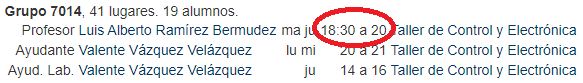
\includegraphics[scale = 0.8]{Ej_gpo_medias_hrs} %width=\textwidth
\caption{\textit{Ejemplo de grupo con medias horas}}
\end{figure}

\item[-] Se tienen materias con múltiples horarios:\url{http://www.fciencias.unam.mx/docencia/horarios/20181/2055/1323}. En estos casos sólo se registran los horarios y salones en los que los profesores imparten su clase, no se toman en cuenta las clases impartidas por los ayudantes.
  
  El profesor imparte su clase los lunes, miércoles y viernes de 13-14hrs en el salón O215, hay una ayudantía los martes y jueves de 13-14hrs en el salón O215 y otra ayudantía los martes de 11-13hrs en el salón 304 (Yelizcalli).
  
Se considera que esta materia inicia a las 13hrs y se imparte en el salón O215.
  
\begin{figure}[H]
\centering
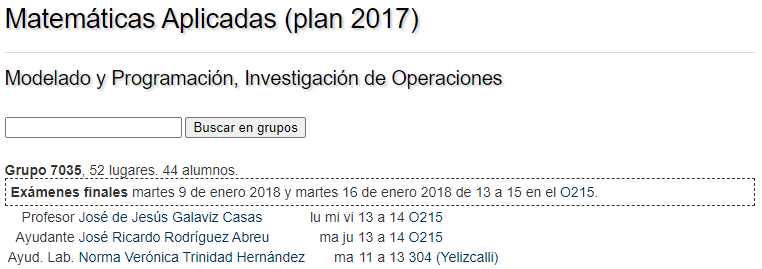
\includegraphics[scale = 0.65]{Ej_gpo_horarios_multiples} %width=\textwidth
\caption{\textit{Ejemplo de grupo con horarios múltiples}}
\end{figure}
  
\item[-] Las materias de inglés no se imparten todos los días de la semana, en algunos casos se imparten clases en línea: \url{http://www.fciencias.unam.mx/docencia/horarios/20202/2017/1135}. Se registran únicamente los horarios de los días en que se imparten las clases presenciales.

\begin{figure}[H]
\centering

\includegraphics[scale = 0.8]{Ej_gpo_ingles} %width=\textwidth
\caption{\textit{Ejemplo de grupo de inglés}}
\end{figure}

\item[-] Se tienen grupos que no tienen la misma estructura que los tipos de grupos \textbf{A}, \textbf{B} y \textbf{C} definidos en la sección \ref{TiposDeGpos}: \url{http://www.fciencias.unam.mx/docencia/horarios/20201/2017/872}, debido a ello el código CSS utilizado no sirve para obtener toda la información que se puede obtener del grupo.

En este caso no se lee adecuadamente el número de alumnos inscritos en el grupo.

\begin{figure}[H]
\centering
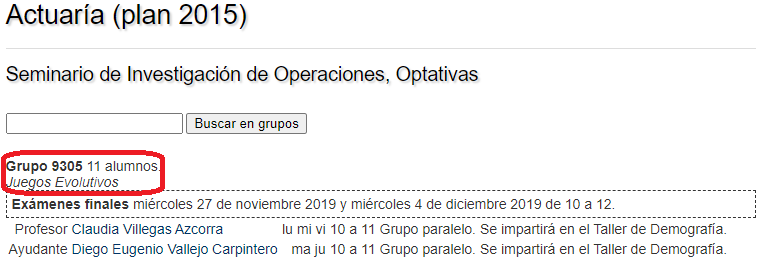
\includegraphics[scale = 0.8]{Ej_gpo_con_estructura_diferente} %width=\textwidth
\caption{\textit{Ejemplo de grupo con estructura diferente}}
\end{figure}

\end{itemize}